\lstset{language=Python} 

\chapter{Aspecto Informático}

\epigraph{“Aim for simplicity in Data Science. Real creativity won’t make things more complex. Instead, it will simplify them.”}{Damian Duffy Mingle}



\section{Introducción al Machine Learning}
%https://en.wikipedia.org/wiki/Portal:Machine_learning

Hasta ahora muchas compañías de todos los tipos y tamaños se han dedicado a obtener un potente sistema de información que les permite almacenar de forma ordenada (o no tanto) todos los datos que se producen en el día a día de la empresa.  

Sin embargo esta estrategia de por sí no sirve de nada, ya que si almacenas datos y no los utilizas nunca, estás desperdiciando tus recursos.  
La ciencia de datos es la disciplina que transforma la información en conocimiento.  
Este conocimiento puede ser utilizado para la toma de decisiones de forma manual o de forma automática.  
El machine learning es el subcampo de la ciencia de datos que se que se centra en hacer que las máquinas aprendan de los datos y puedan realizar 
tareas concretas sin haber sido programadas específicamente para ello.

Actualmente podemos encontrar aplicaciones del machine learning por todas partes:

\begin{itemize}
\item Buscadores web: (Clasificación de contenido)
\item Redes sociales: (Segmentación de clientes en función de los gustos propios y de amigos)
\item Comunicación: (Detección de spam y clasificación automática de la bandeja de entrada)
\item Seguridad: (Detección de malware)
\item Entretenimiento: (Shazam: Reconocimiento de canciones)
\item Marketing: (Netflix: Sistemas de recomendación)
\item Medicina: (Diagnostico de enfermedades)
\item Arte: (Generar imágenes artificialmente) 
\end{itemize}

El Machine Learning no es un concepto nuevo, sin embargo en los últimos años ha tenido un gran auge. Una de las  razones principales de este auge es  el  aumento  en  la  capacidad  de  procesamiento  y  la  disminución  de  los  costes  del mismo, permitiendo así que pueda estar al alcance de todos.

Aquí podemos ver el interés en el machine learning a nivel global utilizando Google Trends:
\begin{center}
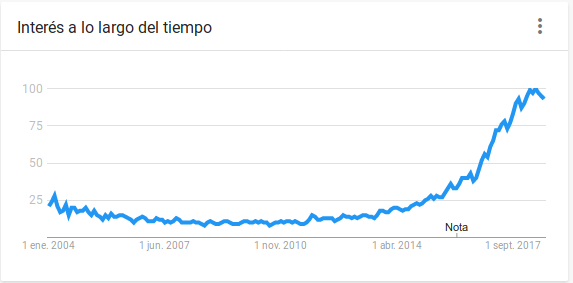
\includegraphics[scale=0.7]{./img/ml_google_trends.png} 
\end{center}

\begin{definicion}
\emph{Machine Learning}\\
Campo  de  estudio  que  da  a  los  ordenadores  la  habilidad  de  aprender  sin  la  
necesidad de ser explícitamente programados. 
Arthur Samuel, 1959
\end{definicion}

\pagebreak
\subsection{Tipos de problemas en Machine Learning}
Hay tres tipos de problemas de machine learning: \textbf{Aprendizaje supervisado}, \textbf{Aprendizaje no supervisado} y \textbf{Aprendizaje por refuerzo}.  

\subsection{Aprendizaje Supervisado}
El objetivo principal del aprendizaje supervisado es construir un modelo a partir de un conjunto etiquetado de \textit{datos de entrenamiento} que nos permita hacer predicciones sobre los datos sin etiquetar que vengan en el futuro.  
Se llama aprendizaje supervisado porque la clave del paradigma radica en tener datos \textit{etiquetados} a priori.  
Hay dos tipos de problemas que se resuelven mediante aprendizaje supervisado:  
\textbf{Clasificación} y \textbf{Regresión}.

\subsection{Aprendizaje No Supervisado}
En el aprendizaje supervisado conocemos la \textit{respuesta correcta} de antemano cuando entrenamos nuestro modelo. En el aprendizaje no supervisado, por contra, estamos tratando con datos sin etiquetar o con datos con \textit{estructura desconocida}. Usando aprendizaje no supervisado podemos explorar la estructura de nuestros datos y extraer información util observando únicamente similitudes y diferencias entre los datos para poder agruparlos de forma que salgan a relucir posibles patrones ocultos en los datos.  
La técnica más popular dentro del aprendizaje no supervisado es el \textit{clustering}.
Este método se utiliza cuando se necesita clasificar las instancias de datos pero no se conocen previamente las categorías. Esta agrupación permite construir grupos (\textit{cluster}) de forma automática para clasificar de una forma lógica aun sin conocer las clases de antemano. 

Un ejemplo clásico es examinar los datos de ventas de una compañía para obtener grupos de clientes similares.


\subsection{Aprendizaje por refuerzo}
En el aprendizaje por refuerzo, el objetivo consiste en desarrollar un sistema (\textit{un agente}) que mejore su rendimiento basandose en interacciones con el entorno. Como la forma de aprender del entorno consite en la nueva incorporación de datos acompalañados de una medida de la \textit{función de recompensa}. Podemos pensar en el aprendizaje por refuerzo como un tipo de aprendizaje supervisado. Sin embargo en el aprendizaje por refuerzo esta etiqueta que acompaña a los nuevos datos no es una clase, como ocurre en el aprendizaje supervisado, sino que es una medida de como de bien o mal se está comportando el agente (valor de la función de recompensa asociado a los nuevos datos).  A traves de la interacción con el entorno un agente puede utilizar aprendizaje por refuerzo para aprender una serie de acciones que maximizen su recompensa mediante ensayo-error o mediante un plan deliberado.  

Un ejemplo clásico de aprendizaje por refuerzo es un programa que juegue a algún juego como el ajedrez. En este caso, el agente decide la jugada basandose en el estado actual del tablero (entorno) y la recompensa puede determinarse como una función que evalua cada situación y que lógicamente asigna la máxima puntuación a ganar y la mínima a perder.


\section{Resolviendo problemas con Aprendizaje Supervisado}
\subsection{Método de Regresión}
Este  método  se  utiliza  para  predecir  el  valor  de  un  atributo  continuo.  Consiste  en encontrar la mejor ecuación que atraviese de forma óptima un conjunto de puntos (n-dimensiones).  
Esta mejor ecuación se va a buscar dentro de una familia de funciones, de esta forma hablaremos de \textit{Regresión Lineal}, \textit{Regresión Logistica} etc...  
En estos métodos lo único que cambiamos es la familia de funciones, aunque también se pueden añadir mecanismos de regularización.


Supongamos que tenemos dos variables aleatorias $X$ e $Y$:
\begin{center}
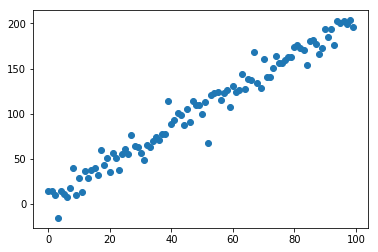
\includegraphics[scale=0.7]{./img/reg_lin_data.png}
\end{center}
Queremos buscar la mejor función lineal que exprese $Y$ como función de $X$:  
Aplicando regresión lineal obtenemos una función lineal $LM(x) = w_0 + w_1x$ tal que $LM(x) \simeq  Y(X)$ 
\begin{center}
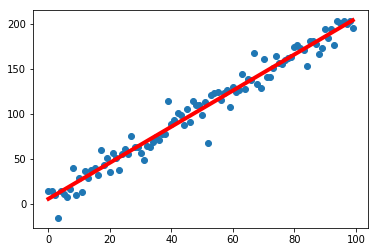
\includegraphics[scale=0.7]{./img/reg_lin_fit.png}
\end{center}

De esta forma ahora podríamos predecir el valor de nuevos datos colocandolos sobre la línea roja en la posición que les corresponda.  
Es decir: $y_{pred} = LM(X_{new})$

\subsection{Método de Clasificación}

Este método se utiliza para predecir a que clase pertenece una determinada instancia a partir de unas caraterísticas determinadas.  
El tipo más simple de clasificación es la clasificación binaria mediante un clasificador lineal:

Ejemplo: 
Supongamos que tenemos datos pertenecientes a dos clases (la clase violeta y la clase amarilla):
\begin{center}
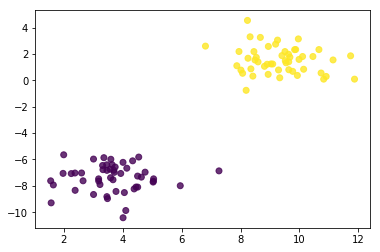
\includegraphics[scale=0.7]{./img/class_lin_data.png}
\end{center}
Queremos buscar la mejor función lineal que separe ambas clases:
\begin{center}
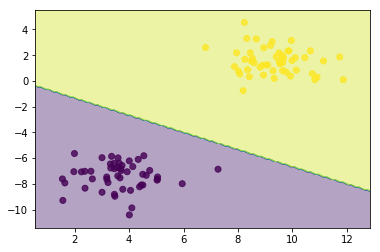
\includegraphics[scale=0.7]{./img/class_lin_fit.png}
\end{center}

\pagebreak

\subsection{Iris: El problema de clasificación más clásico}

En 1936 Ronlad Fisher anotó la colección de datos \textit{Iris}, en el que cuantificó varias mediciones taxonómicas de las flores de tres especies de Iris:

\begin{figure*}[!h]
$\begin{array}{rl}
    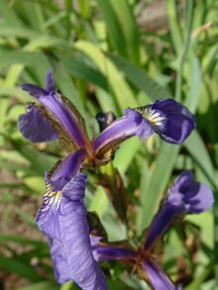
\includegraphics[scale=0.3, width=0.5\textwidth]{./img/Iris_setosa.png} &
    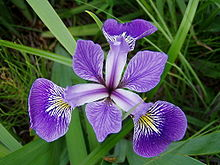
\includegraphics[width=0.5\textwidth]{./img/Iris_versicolor.jpg}\\
    \multicolumn{2}{c}{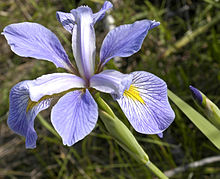
\includegraphics[width=0.5\textwidth]{./img/Iris_virginica.jpg}}
\end{array}$
\caption[Especies de Iris.]{\label{fig:label}Especies de Iris.}
\end{figure*}

\pagebreak
Podemos establecer como variables la longitud del sépalo y la longitud del pétalo y obtenemos una representación en 2D del conjunto de Fisher:

\begin{center}
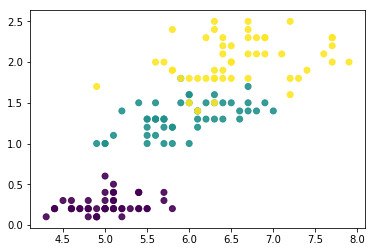
\includegraphics[scale=0.7]{./img/fisher_data.png}
\end{center}

Y podemos establecer muchos tipos de clasificadores:

El clasificador lineal que utilizamos antes se vería de este modo:

\begin{center}
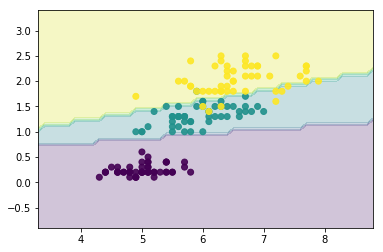
\includegraphics[scale=0.7]{./img/fisher_lin.png}
\end{center}

Pero podemos utilizar tambien clasificadores de tipo Boosting, concretamente el Gradient Boosting Machine, del que hablaremos más adelante y que ocupará la mayor parte del trabajo:

\begin{center}
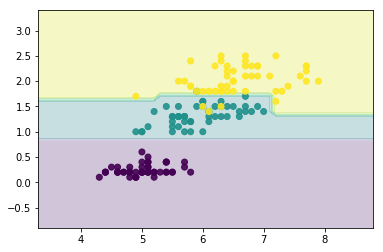
\includegraphics[scale=0.7]{./img/fisher_gbm.png}
\end{center}




\section{El flujo de trabajo para clasificación}

Todos los problemas de clasificación parten de un conjunto de datos etiquetados. Y el objetivo es construir una función que acepta nuevos datos con la misma estructura que en el conjunto inicial, pero sin etiqueta, y devuelve la etiqueta que considera que debe ser la correcta.  

Lo primero, antes de nada es separar el dataset en datos de entrenaminento (training dataset) y en datos de test (test dataset).  
Los datos de test se guardarán hasta el final sin hacer nada sobre ellos y se trabajará únicamente con los datos de entrenamiento.  
Para construir un modelo de calidad, primero deben \textbf{preprocesarse} los datos de entrenamiento, es decir, normalizarlos, escalarlos, aplicar transformaciones, seleccionar qué variables son importantes y cuales no...
Este es un subcampo bastante amplio llamado \textit{Ingeniería de Características}.  
Normalmente el preprocesamiento es la parte que más tiempo requiere y a la que el cientifico de datos más esfuerzo debe dedicarle.

Una vez se han preprocesado los datos de entrenamiento se utilizarán para \textbf{ajustar un modelo}, es decir, se construirá un modelo mediante un algoritmo de aprendizaje.

Una vez el modelo se ha construido llega el turno de \textbf{evaluar la calidad del modelo}, lo mejor es utilizar cross validation con los datos de entrenamiento para evaluarlo y dejar los de test únicamente para evaluar los modelos que creemos que son buenos.  
Existen técnicas para ajustar los parámetros empíricamente como por ejemplo \textit{gridsearch}.

Una vez tenemos un modelo de calidad podrá utilizarse para \textbf{predecir nuevos datos} y nuestro trabajo volverá a empezar para mejorar el modelo si así lo consideramos necesario.  

\begin{center}
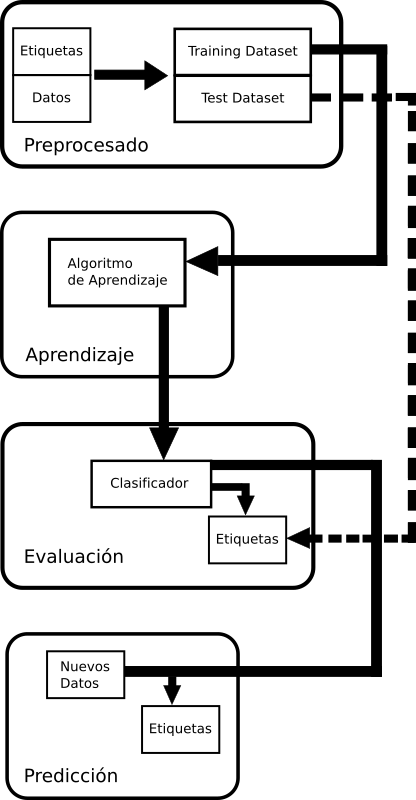
\includegraphics[scale=0.7]{./img/workflow.png}
\end{center}

\pagebreak

\section{Uso de Python para Machine Learning}
En este caso vamos a utilizar Python, debido a que actualmente se está convirtiendo en el lenguaje más utilizado para ciencia de datos, además de estar ganando terreno a muchos otros lenguajes clásicos debido a la enorme cantidad de librerías que existen para Python.  
La mayor alternativa a Python es el lenguaje estadístico R.  
No obstante un cientifico de datos debería conocer ambos lenguajes ya que R es muy potente a la hora de hacer un buen análisis exploratorio de forma rápida y eficaz.  
En Python también es posible trabajar como con R de forma rápida e interactiva utilizando Jupyter Notebook.  

Para lo que nos ocupa nos centraremos en utilizar las principales liberías de Python para Machine Learning:  

\begin{itemize} 
	\item{\textit{numpy}: Es una libería de cálculo numérico para Python, se encarga de que las opereciones computacionalmente intensivas con matrices se hagan con rutinas C muy eficientes en lugar de directamente interpretadas con Python}
	\item{\textit{pandas}: Es una libería para importar y exportar datos en Python, además con pandas es muy facil manejar grandes tablas de forma cómoda ya que está construida sobre \textit{numpy}} 
	\item{\textit{scipy}: Es otra colección de rutinas en Fortran y C para agilizar los cálculos científicos} 
	\item{\textit{scikit-learn}: Está contruida sobre \textit{numpy} y \textit{scipy} y tiene una gran cantidad de herramientas para poder completar el flujo de trabajo de un problema de machine learning sin necesidad de otras librerías en la mayoría de los casos sencillos} 
	\item{\textit{xgboost}: Es una librería que contiene la implementación del algoritmo XGBoost, el algoritmo de boosting más utilizado en la actualidad} 
	\item{\textit{matplotlib}: Es una librería para visualización de gráficos} 
\end{itemize}

\subsection{Instalación de Python y de paquetes}
Python está disponible para los tres grandes sistemas operativos (Linux, Microsoft Windows y Mac OS X).  
En la mayoría de distribuciones Linux modernas Python viene instalado por defecto en su versión moderna (Python3).  
En Mac no obstante aún viene por defecto la versión 2.7 (Python antiguo).
Lo ideal en este caso es instalar Python3 con un alias (python3) y utilizarlo, pero sin desinstalar el Python del sistema, ya que el sistema operativo utiliza internamente la versión 2.7 para algunas tareas.  
En Windows Python no viene instalado por defecto en ninguna versión por lo que hay que descargarlo de la web oficial: https://www.python.org  

Todo el código que se ha utilizado en este proyecto está escrito para Python3 y debería funcionar en todas las versiones superiores a la 2.7.10  

Para instalar paquetes en Python utilizaremos su gestor de paquetes \textit{pip}.

\textit{pip install nombre\_paquete}

En nuestro caso vamos a instalar los paquetes básicos, que ya hemos comentado antes, para probar el flujo de trabajo en machine learning.  
Más adelante profundizaremos en la utilización de los algoritmos de boosting.  

\subsection{Jupyter Notebook}
Merece especialmente la pena utilizar Jupyter notebook, ya que podemos trabajar con Python de forma interactiva y generar informes de forma rápida y reproducible por otras personas.  
Jupyter Notebook levanta un servidor web en nuestra máquina y nos podemos conectar vía navegador web a localhost. En este punto Jupyter está sirviendo una aplicación web en la que podemos escribir bloques de código python y enviarlos a ejecutarse con una instancia de python (el kernel de jupyter).

También tiene opciones para exponer el notebook a la red de forma segura, por lo que podríamos utilizar jupyter notebook en un servidor con gran potencia de procesamiento y trabajar de forma remota

Jupyter Notebook viene de serie si utilizamos \textbf{Anaconda} para instalar Python junto con todas las herramientas básicas de ciencia de datos.

\section{Algoritmos de Boosting}

El boosting es un tipo particular de método para generar un ensemble, este ensemble consiste en un conglomerado de  clasificadores débiles (que son solo un poco mejor que la asignación aleatoria) que actúan de forma conjunta para construir un clasificador fuerte (de gran calidad). Un ejemplo típico de clasificado débil es un arbol de una sola hoja.  
En boosting se va construyendo el clasificador de forma iterativa, como ya mencionamos en la sección matemática.  
Las instancias que no han sido bien clasificadas en la iteración anterior adquieren una mayor importancia para la siguiente iteración. Podríamos decir que el algoritmo de boosting va concentrandose en acertar las instancias más dificiles conforme avanza en su proceso iterativo.  

Este proceso iterativo se ve reflejado en la siguiente ilustración:
\begin{center}
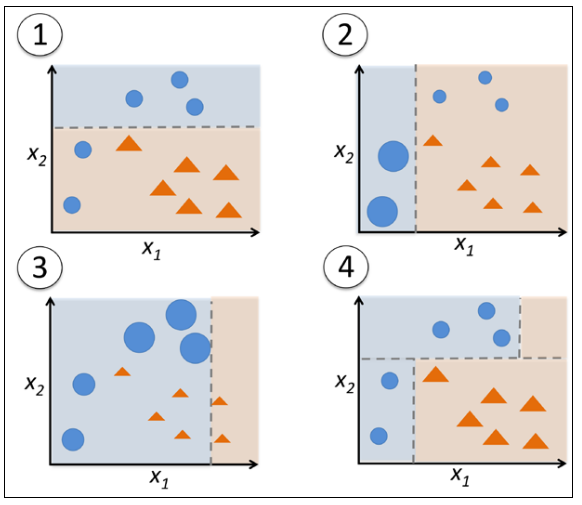
\includegraphics[scale=0.7]{./img/adaboost.png}
\end{center}

\subsection{Adaboost}

Adaboost es el algoritmo de boosting más simple.  
En Python puede implementarse definiendo un clasificador débil que actúe como base y construyendo el clasificador adaboost en base a él.  

En el anexo podemos observar el mismo ejemplo del cáncer de mama aplicando Adaboost con árboles de una sola hoja como hemos explicado anteriormente.

\subsection{Extreme Gradient Boosting - XGBoost}
Adaboost es una forma de boosting simple pero poco eficaz en ejemplos reales.  
En la actualidad el algoritmo de boosting más famoso es XGBoost, una implementación muy eficiente del Gradient Boosting que aprovecha al máximo los recursos hardware disponibles mediante paralelización.  

Podemos ver la utilización de XGBoost en el anexo.

\section{Ruido de clase, Regularización, Underfing y over-fitting}
Se denomina ruido de clase a las instancias mal clasificadas en el conjunto de entrenamiento.
Estas instancias deben ser eliminadas a toda costa de nuestro conjunto de entrenamiento, pero el problema es que no sabemos cuales son ruidosas y cuales no.  
Lo que si está en nuestra mano es desconfiar de instancias cuya clase no concuerde con la que según el clasificado debería tener. Esta aproximación consistiría en aplicar un filtro de ruido, normalmente basado en KNN para eliminar del dataset aquellas instancias cuyos $k$ vecinos más cercanos tengan una clase diferente.  

La regularización es una técnica que consiste en conseguir que un clasificador sea capaz de funcionar adecuadamente en datos que nunca ha visto, es decir que no solo se ciña al conjunto de aprendizaje sino que sea capaz de generalizarlo.  
Para ello lo que la regularización hace es limitar la complejidad del modelo, por ejemplo penalizando a los clasificadores que utilizan más parámetros en su ajuste.  
Por ejemplo, en un árbol de decisión, la regularización puede consistir en penalizar a los árboles que tienen más nodos hoja.


\subsection*{Underfiting / over-fitting}

Los conceptos de under-fitting y over-fitting son conceptos contrapuestos y hacen referencia a los casos en los que estamos tratando el problema como algo demasiado general (under-fitting) o por el contrario estamos cayendo en over-fitting, ciñéndonos demasiado a los datos de entrenamiento y aprendiendo comportamientos aleatorios en un modelo muy complejo que no se ajusta a la realidad (la cual es más simple muchas veces).  

La siguiente imagen es muy esclarecedora de qué es el over-fitting y el under-fitting

\begin{center}
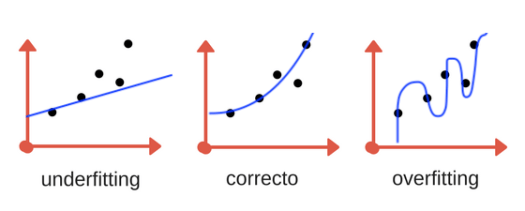
\includegraphics[scale=0.7]{./img/generalizacion-machine-learning.png}
\end{center}

En los casos en los que nuestros datos son ruidosos debemos tener especial cuidado con no caer en el over-fitting, ya que aprenderíamos el ruido y nos sería muy difícil acertar en las predicciones con nuestro modelo una vez lo llevemos a predecir la realidad en un entorno productivo.

Es por esto que vamos a prestar especial atención a cómo aplicar factores de regularización al algoritmo XGBoost.

\section{Regularización en XGBoost}

En XGBoost los principales parámetros para regularización son:

\textbf{min\_child\_weight}
Define la suma mínima de los pesos de todas las observaciones que se requiere para crear un nuevo nodo en el árbol.
Si establecemos un valor alto estaremos evitando crear nodos que se ajusten a conductas demasiado específicas de un pequeño grupo de observaciones en nuestro conjunto de datos de entrenamiento.
Sin embargo si establecemos un valor demasiado amplio vamos a descartar prácticamente todo nuestro dataset, salvo las conductas generales, cayendo por tanto en under-fitting.


\textbf{max\_depth} 
La profundidad máxima de una rama de un árbol.
Si no permitimos ramas muy profundas estamos evitando el over-fitting , ya que el árbol será incapaz de aprender las conductas que sean demasiado específicas.

\textbf{gamma}
Es el multiplicador de Lagrange que acompaña a la función de pérdida:
Un nodo se divide solamente cuando el resultado de la división conduce a una reducción de la función de pérdida. Gamma es proporcional a la magnitud de la reducción de la función de pérdida necesaria para que se produzca la división. Por tanto debe elegirse un gamma u otro dependiendo de cuál sea nuestra función de pérdida.

\textbf{lambda}
Es el factor de regularización L2 (análogo a la regresión Ridge)

\textbf{alfa}
Es el factor de regularización L1 (análogo a la regresión Lasso)








































